\documentclass[10pt]{beamer}

\usetheme[progressbar=frametitle]{metropolis}
\usepackage{appendixnumberbeamer}

\usepackage{booktabs}
\usepackage[scale=2]{ccicons}

\usepackage{pgfplots}
\usepgfplotslibrary{dateplot}


\usepackage{xspace}
\newcommand{\themename}{\textbf{\textsc{metropolis}}\xspace}
\usepackage{minted}

\title{YACRA - Yet Another Code Retrieval Approach}
\subtitle{Um estudo preliminar sobre o uso de uma arquitetura deep learning para seleção de respostas no problema de recuperação de código-fonte}
% \date{\today}
\date{}
\author{Marcelo de Rezende Martins\inst{1}, Marco Aurélio Gerosa\inst{2}}
\institute{\inst{1}Instituto de Pesquisas Tecnológicas
  (IPT) \and \inst{2}Northern Arizona University (NAU)}
% \titlegraphic{\hfill\includegraphics[height=1.5cm]{logo.pdf}}

\begin{document}

\maketitle

\begin{frame}{Índice}
  \setbeamertemplate{section in toc}[sections numbered]
  \tableofcontents%[hideallsubsections]
\end{frame}

\section[Introdução]{Introdução}

\begin{frame}[fragile]{Definição}

A tarefa do \textit{code retrieval} ou recuperação de trecho de código-fonte consiste em:
 
\emph{Dado uma descrição em linguagem natural, recuperar o trecho de código-fonte mais relevante, tal que os desenvolvedores possam encontrar rapidamente os trechos de código que atendam as suas necessidades. \cite{Chen-bi-variational-autoencoder:2018}}
 
\end{frame}
\begin{frame}[fragile]{Definição}
  \textbf{Code Retrieval}: Dada uma questão em linguagem natural $Q$, um modelo $F_{r}$ irá aprender a recuperar o trecho de código-fonte $C^{*} \in \mathbb{C}$ com a maior pontuação \cite{yao-2018}:

\begin{equation}\label{eq:code-retrieval}
C^{*} = \underset{C \in \mathbb{C}}{argmax}\text{ } F_{r}(Q , C)
\end{equation}
  
\end{frame}

\section{Abordagem}

\begin{frame}{Hipótese inicial}
	\textbf{Hipótese inicial:} \emph{software é uma forma de comunicação humana e tem propriedades estatísticas similares a corpora de linguagem natural \cite{Allamanis:2018:SML}}
\end{frame}

\begin{frame}{Joint embedding}
	Seja $\mathbb{Q}$ o conjunto formado pelas questões e $\mathbb{C}$ o conjunto composto por trechos de código-fonte \cite{Gu-deep-code-search:2018}:
	
    \begin{equation}
        \mathbb{C} \xrightarrow{\mathbb{E}_{c}} \mathbb{V}_{c} \rightarrow \mathbb{J}(\mathbb{V}_{c}, \mathbb{V}_{q}) \leftarrow \mathbb{V}_{q} \xleftarrow{\mathbb{E}_{q}} \mathbb{Q}
    \end{equation}
\end{frame}


\begin{frame}{Forma de aprendizagem}
	Função de perda \textit{hinge} \cite{tan-lstm-qa, Gu-deep-code-search:2018}:
	
    \begin{equation}
    L = max(0, m - \mathbb{J}(q_{i}, c_{i}^{+}) + \mathbb{J}(q_{i}, c_{i}^{-}))   
    \end{equation}
\end{frame}





\begin{frame}{Arquitetura}
	\begin{figure}[h]
    \centering
    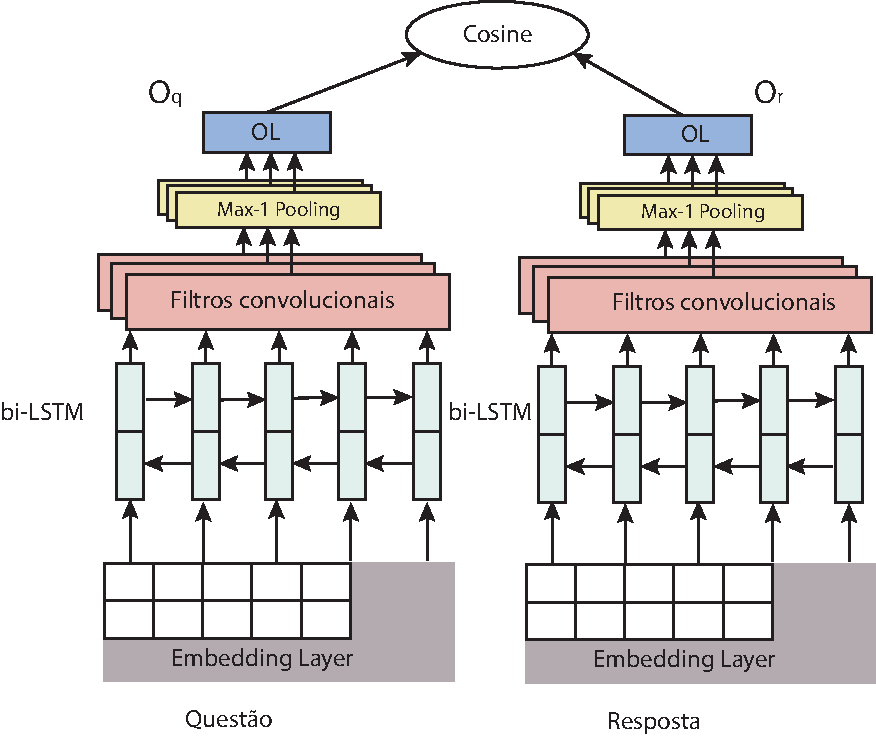
\includegraphics[width=0.7\textwidth]{ArquiteturaBiLSTM.pdf}
    \caption{Figura adaptada do \cite{tan-lstm-qa}.}
    \label{fig:arquitetura-bi-lstm}
\end{figure}
\end{frame}


\section{Experimento}

\begin{frame}[fragile]{Treinamento}
      \begin{table}[h]
\centering
\begin{tabular}{ p{3cm} r  }
 \hline
 \textbf{Amostras} & \textbf{Quantidade de $(q_{i}, c_{i}^{+})$}\\
 \hline
 Treinamento & $60.083$\\
 
 DEV & $1.085$ \\
 
 EVAL & $1.084$\\
 \hline
 \textbf{Total} & $\textbf{62.252}$\\
 \hline
\end{tabular}
\caption{Divisão das amostras para treinamento conforme os critérios adotados por \cite{iyer-etal-2016-summarizing}.}
\label{table:divisao-amostras}
\end{table}
\end{frame}

\subsection{Avaliação}
\begin{frame}{Resultados preliminares}
  \begin{table}[h]
\centering
\begin{tabular}{ p{3cm} p{3cm} }
 \hline
 \textbf{Modelos} & \textbf{Resultados (MRR)}\\
 \hline
 Embedding & $0,52 \pm 0,01$\\
 
 CNN & $0,58 \pm 0,01 $ \\
 
 \textbf{bi-LSTM-CNN} & $\textbf{0,60} \pm \textbf{0,02}$\\
 \hline
\end{tabular}
\caption{Resultado preliminar do modelo bi-LSTM-CNN proposto em comparação a outros dois modelos (CNN e Embedding). Estes resultados foram obtidos a partir da amostra EVAL.}
\label{table:resultados-preliminares}
\end{table}
\end{frame}

\begin{frame}{Histograma das posições dos trechos de código-fonte relevantes}
  \begin{figure}[h]
    \centering
    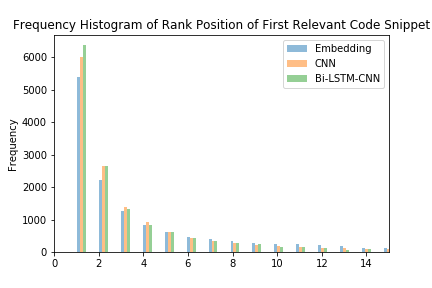
\includegraphics[width=1\textwidth]{histogram_results.png}
    \caption{Figura adaptada do \cite{tan-lstm-qa}.}
    \label{fig:histogram-results}
\end{figure}
\end{frame}

\begin{frame}[fragile]{Exemplos}
        \alert{Python and appending items to text and \colorbox{green}{excel} \colorbox{green}{file}}\footnote{{\tiny \url{https://stackoverflow.com/questions/24593478/python-and-appending-items-to-text-and-excel-file}}}
        \metroset{block=fill}
        \begin{exampleblock}{BiLSTM-CNN}
        \begin{minted}[breaklines,fontsize=\scriptsize, escapeinside=||]{python}
Yvalues = [1, 2, 3, 4, 5]
file_out = |\colorbox{green}{open}|('file.csv','wb')
mywriter=|\colorbox{green}{csv}|.|\colorbox{green}{writer}|(file_out, delimiter = '\n')
mywriter.|\colorbox{green}{writerow}|(Yvalues)
file_out.close()
        \end{minted}
        \end{exampleblock}
        \begin{alertblock}{CNN}
        \begin{minted}[breaklines,fontsize=\scriptsize, escapeinside=||]{python}
import csv

with |\colorbox{green}{open}|("output.csv", "wb") as f:
    writer = |\colorbox{green}{cwv}|.|\colorbox{green}{writer}|(f)
    writer.|\colorbox{green}{writerows}|(a)
    \end{minted}
    \end{alertblock}
    
\end{frame}




{\setbeamercolor{palette primary}{fg=black, bg=yellow}
\begin{frame}[standout]
  Perguntas?
\end{frame}
}

\appendix


\begin{frame}[allowframebreaks]{Referências}

  \bibliography{demo}
  \bibliographystyle{abbrv}

\end{frame}

\end{document}
